\aufgabenbereich{Fließkommaarithmetik}
Für diesen Aufgabenbereich nutzen wir den IEEE 754 Standard für Minifloats.\\
D.h. wir benutzen eine 8 Bit Darstellung mit einem Vorzeichen-,  3 Manitssen- und 4 Exponentbits.

\subsection{}
Wie groß ist der Bias unserer Darstellung?\makeinlineanswerbox{1}{6cm}\\[0.3cm]
Was ist der Bias für eine Fließkommzahl\\[-0.2cm]mit einem Exponent der Länge 6? \makeinlineanswerbox{1}{6cm}\\
\subsection{}
Konvertieren Sie diese Sonderfälle in Fließkommadarstellung:
\begin{center}
	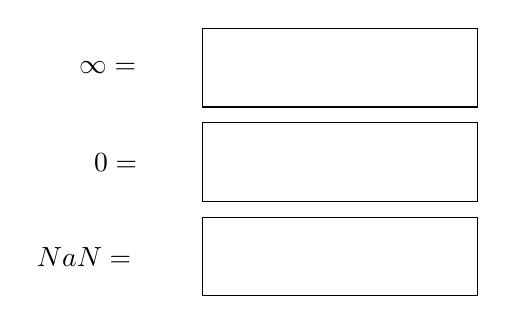
\begin{tikzpicture}
	\node at (0.3,2.4) {$\infty =$};
	\node at (0.4,1.2) {$0 =$}; 
	\node at (0,0) {$NaN=$};
	
	\draw (1.5,1.9) rectangle (5,2.9);
	\draw (1.5,0.7) rectangle (5,1.7);
	\draw (1.5,-0.5) rectangle (5,0.5);
	\end{tikzpicture}
\end{center}
\subsection{}
Bestimmen sie die einzelnen Bestandteile der Fließkommazahl $11011100_{(2F)}$:
\begin{center}
	\tikz[baseline=-1ex]{ \node at (0,0) {$V=$};
		\draw (1,-0.5) rectangle (4,0.5);} \\[1ex]
	\tikz[baseline=-1ex]{ \node at (0,0) {$E=$};
		\draw (1,-0.5) rectangle (4,0.5);} \\[1ex]
	\tikz[baseline=-1ex]{ \node at (0.05,0) {$M=$};
		\draw (1,-0.5) rectangle (4,0.5);} 
\end{center}
\subsection{}
Konvertieren Sie $11011100_{(2F)}$ in eine Dezimalzahl:\\
\makeanswerbox{7}
\subsection{}
Addieren Sie $01011100_{(2F)}$ und $01001000_{(2F)}$ mittels Fließkommaarithmetik:\\
\makeanswerbox{7}
\subsection{}
Multiplizieren Sie $01011100_{(2F)}$ und $00111100_{(2F)}$ mittels Fließkommaarithmetik:\\
\makeanswerbox{7}
\subsection{}
Stellen sie $1_{10}$ in Fließkommaschreibweise da:\\
\makeanswerbox{1}\\[0.3cm]
Zeigen Sie anhand eines Beispiels, dass man durch das kontinuierliche Addieren von $1_{10}$ auf eine beliebige Fließkommazahl F ($\neq \infty$) niemals $\infty$ erreicht.\\
\makeanswerbox{7}